\begin{frame}{Limitations of Perceptrons}
    \begin{itemize}
        \item If the data is not separable, the training algorithm may not terminate.
        \item Test accuracy rises at first, but then starts falling.
        \item We should have a sufficiently small learning rate $\eta$
    \end{itemize}
	\begin{figure}[H]
		\centering
		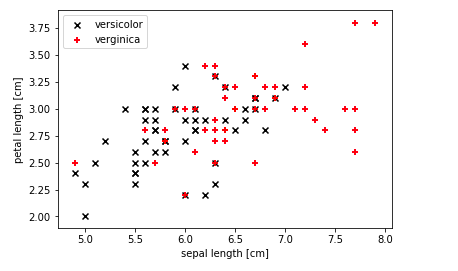
\includegraphics[width=0.6\textwidth]{Images/Not_Separable_Data.png}
		\caption{Not separable data \cite{https://vitalflux.com/how-know-data-linear-non-linear/}.}
	\end{figure}
\end{frame}

\begin{frame}{Multi-Layered Perceptron}
    \begin{itemize}
        \item Why Should we do?
        \begin{itemize}
            \item One of the main weaknesses of linear models are that they are linear and they ran into problem when the data has non-linear relations.
            \item So we take our biological inspiration further by chaining together perceptrons.
        \end{itemize}
    \end{itemize}
	\begin{figure}[H]
		\centering
		
\includegraphics[width=0.5\textwidth]{Images/Brain.png}
		\caption{Inspiration \cite{https://www.pngwing.com/en/free-png-xzwgm}.}
	\end{figure}
\end{frame}

\begin{frame}{Learning with hidden units}
    \begin{itemize}
        \item Networks without hidden units are very limited in the
input-output mappings they can model.
        \begin{itemize}
            \item More layers of linear units do not help. Its still linear.
            \item Fixed output non-linearities are not enough
        \end{itemize}
        \item We need multiple layers of adaptive non-linear hidden
units. This gives us a universal approximator.
        \begin{itemize}
            \item We need an efficient way of adapting all the weights,
not just the last layer. This is hard. Learning the
weights going into hidden units is equivalent to
learning features.
            \item Nobody is telling us directly what hidden units should
do.
        \end{itemize}
    \end{itemize}
    \begin{figure}[H]
		\centering
		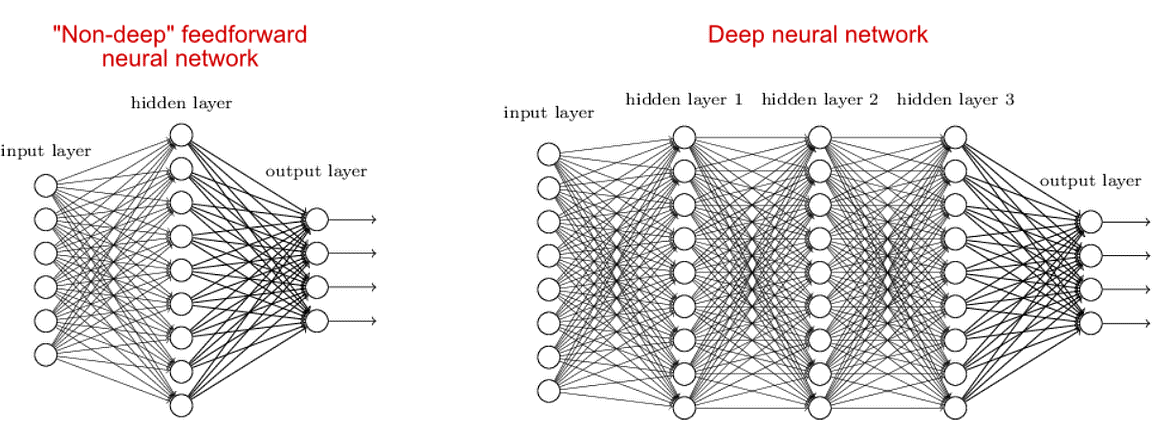
\includegraphics[width=0.4\textwidth]{Images/MLP1.png}
		\caption{Multi layer perceptron \cite{https://www.projectpro.io/article/deep-learning-algorithms/443}.}
	\end{figure}
\end{frame}

\begin{frame}{XOR Example}
    \begin{itemize}
        \item A Perceptron cannot learn the XOR function. 
        \begin{itemize}
            \item Positive cases: $(1, 0) -> 1; (0, 1) -> 1$
            \item Negative cases: $(1, 1) -> 0; (0, 0) -> 0$
            \item ?I need to draw a perceptron myself?
        \end{itemize}
    \end{itemize}
\end{frame}

\begin{frame}{Multi-Layer perceptron neural architecture}
    \begin{itemize}
        \item In a typical MLP network, the input units ($X_i$) are fully
connected to all hidden layer units ($Y_j$) and the hidden layer
units are fully connected to all output layer units ($Z_k$).
        \item Each of the connections
between the input to hidden
and hidden to output layer
units has an associated weight
attached to it ($W_{ij}$ or $W_{jk}$)
        \item The hidden and output layer
units also derive their bias
values ($b_j$ or $b_k$) from
weighted connections to units
whose outputs are always 1
(true neurons)
    \end{itemize}
	\begin{figure}[H]
		\centering
		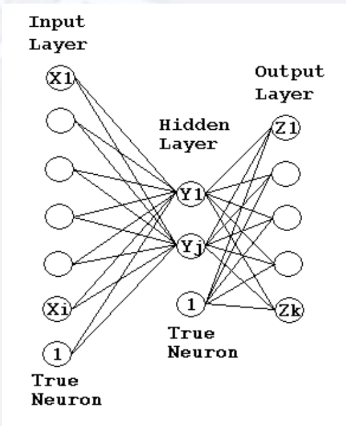
\includegraphics[width=0.3\textwidth]{Images/MLP2.png}
		\caption{MLP Architecture \cite{Gonna Replace It/}.}
	\end{figure}
\end{frame}

\begin{frame}{Two-layer MLP}
    \begin{itemize}
        \item Two-layer networks are Universal function approximators.
        \begin{itemize}
            \item It can approximate any continuous function on a bounded subset of D-dimensional space.
        \end{itemize}
        \item How many hidden units needed then?
        \begin{itemize}
            \item 
        \end{itemize}
    \end{itemize}
\end{frame}

\begin{frame}{Two-layer MLP}
    \begin{itemize}
        \item $X_i = input[i]$
        \item $Y_j = f(b^1_j + \sum{X_i W^1_{ij}})$
        \item $Z_k = g(b^2_k + \sum{Y_j W^2_{jk}})$
    \end{itemize}
	\begin{figure}[H]
		\centering
		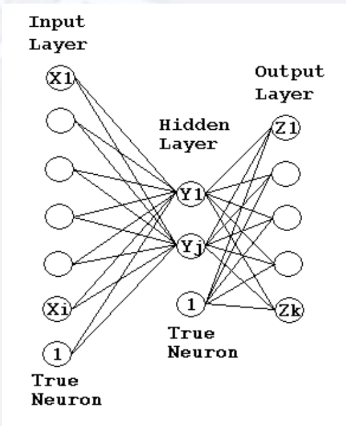
\includegraphics[width=0.3\textwidth]{Images/MLP2.png}
		\caption{MLP Architecture \cite{Gonna Replace It/}.}
	\end{figure}
\end{frame}

\begin{frame}{Non-linearity}
\begin{itemize}
    \item 1-Layer MLP: $Z = g(Wx)$
    \item 2-Layer MLP: $Z = g(W_2f(W_1x))$
    \item 3-Layer MLP: $Z = g(W_3f_2(W_2f_1(W_1x)))$
    \item What does deep mean?
    \begin{itemize}
        \item In any directed acyclic graph (DAG) "Depth" is the length of the longest path from a source to a sink
    \end{itemize}
\end{itemize}
    
\end{frame}

\begin{frame}{Learning by perturbing weights}
    \begin{itemize}
        \item Randomly perturb one weight and see
if it improves performance. If so, save
the change.
        \begin{itemize}
            \item Very inefficient. We need to do
multiple forward passes on a
representative set of training data
just to change one weight.
            \item Towards the end of learning, large
weight perturbations will nearly
always make things worse.
        \end{itemize}
        \item We could randomly perturb all the
weights in parallel and correlate the
performance gain with the weight
changes.
        \begin{itemize}
            \item Not any better because we need
lots of trials to “see” the effect of
changing one weight through the
noise created by all the others.
        \end{itemize}
    \end{itemize}
\end{frame}

\begin{frame}{Training a MLP}
    \begin{itemize}
        \item Now we need to find the Optimal weights for our network
    \end{itemize}
    \begin{block}{Optimazation}
        \[
            \begin{cases}
                min_{W_N, ..., W_1} \sum_{n=1}^{N} \dfrac{1}{2} (t_n - Z_n)^2 \\
                Z = g(W_Nf_{N-1}(...(W_2f_1(W_1x))...))
            \end{cases}
        \]
    \end{block}
    \begin{itemize}
        \item Loss minimization: replace squared-loss with any other
        \item Regularization:
        \begin{itemize}
            \item traditionally NN's are not regularized.
            \item But you can add a regularization.
        \end{itemize}
        \item Optimization by gradient descent (Not gurantees about optimality)
    \end{itemize}
\end{frame}

\begin{frame}{Training a 2-layered network}
    \begin{block}{2-layered network optimazation term}
        \[
            \begin{cases}
                min_{W_2, W_1} \sum_{n=1}^{N} \dfrac{1}{2} (t_n - \sum{i}{} w^2_if(w^1_ix_n))^2 \\
            \end{cases}
        \]
    \end{block}
    \begin{block}{Equiavantly}
        \[
            \begin{cases}
                min_{W_2, W_1} \sum_{n=1}^{N} \dfrac{1}{2} (t_n - \sum{i}{} w^2h_h{i,n}
                \\
                h_{i,n} = f(w^1_ix_n)
            \end{cases}
        \]
    \end{block}
    \begin{block}{Computing gradients: output layer}
        
    \end{block}
\end{frame}

\begin{frame}{Back Propagation}
    \begin{itemize}
        \item We don’t know what the hidden units ought to do,
but we can compute how fast the error changes as
we change a hidden activity.
        \begin{itemize}
            \item Instead of using desired activities to train the
hidden units, use error derivatives w.r.t. hidden
activities.
            \item Each hidden activity can affect many output units
and can therefore have many separate effects on
the error. These effects must be combined.
            \item We can compute error derivatives for all the
hidden units efficiently.
            \item Once we have the error derivatives for the
hidden activities, its easy to get the error
derivatives for the weights going into a hidden
unit.
        \end{itemize}
    \end{itemize}
\end{frame}

\begin{frame}{Back propagation algorithm}
    \begin{itemize}
        \item Initialize each $W_i$ to some small random value
        \item Until the termination condition is met, Do
        \begin{itemize}
            \item For each training example $<(x_1, ..., x_n), t>$ Do
            \begin{itemize}
                \item Input the instance $(x_1, ..., x_n)$ to the network and compute the network outputs $Z_k$
                \item for each output unit k
                \item $\delta_{pk} = z_k (1-z_k)(t_k-y_k)$
                \item for each hidden unit h in the j layer
                \item $\delta_{j,h} = y_{j,h} (1-y_{j,h}) \sum_{k}{}W^j_{h,k} \delta_{j+1,k}$
                \item for each network weight $W^j_{h,k}$ Do
                \item $W^j_{h,k} = W^j_{h,k} + \Delta^j_{h,k}$ where
                $\Delta^j_{h,k} = \eta \delta_{j,k} x_{i,j}$
            \end{itemize}
        \end{itemize}
    \end{itemize}
\end{frame}

\begin{frame}{Back propagation}
    \begin{itemize}
        \item Gradient descent over entire network weight vector
        \item Easily generalized to arbitrary directed graphs
        \item Will find a local, not necessarily global error minimum
        \begin{itemize}
            \item in practice often works well (can be invoked multiple
                times with different initial weights)
        \end{itemize}
        \item Minimizes error training examples
        

    \end{itemize}
\end{frame}